%%==================================================
%% chapter02.tex for BIT Master Thesis
%% modified by 朱杰
%%==================================================
\chapter{相关工作}
\section{社交网络}
\subsection{社交网络概述}
在维基百科中,社交网络(Social Network)被定义为“由许多节点以及节点间关系构成的一个网络结构。节点通常是指个人或组织(又称社团),社交网络代表各种社会关系”。对社交网络的分析在早期只是针对现实生活中切实的方便调查的关系进行分析。比方说:早期在国外曾有研究人员在研究如何减少政府机构的冗余行政人员以提高办事效率和降低政府开销时,就使用到了社交网络分析这一手段。他们采用私下采访和调查的手段获取了某一政府机关几乎全部工作人员之间的来往接触关系,建立了一张交际网络。通过对这张交际网络的分析发现,其中有些节点在业务流程线上是属于多余的,其功能只是交接两边的节点。对于提高效率而言,分析此网络并减少这样无谓的节点即可有效的降低开销。不像早期的社交网络主要是通过合作关系建立起来的职业网络,如今随着互联网社交媒体的诞生和飞速发展,社交网络逐渐线上化。

本文所指的社交网络特指在线社交网络(下文统称社交网络)。现在人们所说的社交网络一般而言其实就指代在线社交软件,也就是在互联网上与其他人产生联系的一个平台。在线社交媒介主要有即时通讯类软件(比如微信、QQ)、在线社交类软件(比如Facebook、人人网)、微博类软件(比如新浪微博、Twitter)、贴吧类软件(比如百度贴吧、悟空问答、知乎)、博客分享类软件(比如CSDN、简书)、职场关系类软件(比如领英、脉脉)和短视频分享类软件(比如抖音、快手)等等。而社交网络就是在这些社交媒介中抽象虚拟出来的一张网络图,在这张图中,每个个人或者组织抽象为一个节点,而人与人之间的关系或者互动则抽象为边。每个账号在社交媒体上填写的个人信息就是其节点属性,同样节点彼此之间的边上也有着相应的边的属性。这一切就构成了一个社交网络结构。网络虽然都是抽象出来的,但是这些关系却又都是真实的。图\ref{fig:fig2-1}展示了一个简单的社交网络抽象图。

\begin{figure}
  \centering
  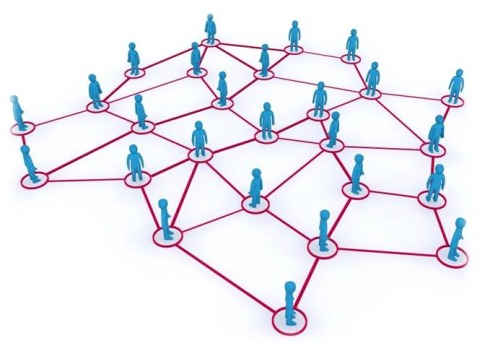
\includegraphics[width=0.75\textwidth]{figures/fig2-1}
  \caption{一个简单的社交网络抽象图}\label{fig:fig2-1}
\end{figure}

% 在种类繁多各色各样的在线社交媒体中,人们的参与度也越来越高。2017年Q3微博财报数据显示,截至2017年9月,微博月活跃用户共3.76亿;2018年1月15日,在广州举行的微信公开课上微信创始人、腾讯高级副总裁张小龙指出微信用户量已超10亿;而国外的Facebook更是早在2017年就已超20亿用户。社交网络具有传播迅速、传播广泛、自发性和言论相对自由等特点。面对这么巨大的用户量,不仅仅是普通个人用户,我们可以发现在诸多知名在线平台上各类官方媒体也都已入驻,以借助传播更加快捷和广泛的在线社交媒介来达到进行宣传等目的。当然,因为用户量的越发增加,在线社交媒介的广泛使用带来的问题也越来越多。这也对社交网络的规范化和整治不断提出挑战。

% 在现在这样的背景下,已经越发明显的出现线上影响线下的这种趋势。在人们享受社交网络带来的乐趣和便利之时,同样也有不法分子为了金钱或其他利益利用社交网络缺乏规范又利于传播等特点进行违法犯罪,包括诈骗、散布暴力恐怖信息或谣言等等。最近国家广电总局也整治了一大批社交媒体,封杀了一系列严重违规的软件,即使是今日头条、抖音、快手这样的大公司也面临着很大的危机,被勒令整改。因此,为了更好的利用社交网络给人们带来的便捷,同时又能避免产生危害,就产生了社交网络分析(Social Network Analysis)这一研究领域。它是一门横跨信息学、数学、计算机技术、社会学、管理学和心理学等学科的交叉科学,主要研究的是社交网络的网络结构和其演化、社交网络中的群体及其互动、社交网络中的信息及其传播。

\subsection{社交网络的统计特性}

因为社交网络的本质其实就是一个由节点(人或组织)和边(社会关系)组成的图结构,所以说社交网络模型之中的很多概念都是来源于图论。在这一小节中,将会简单介绍社交网络中常用的几种统计概念,包括节点的度及其分布、网络密度、平均路径长度、边的介数和聚类系数。这些统计概念或多或少都旨在反映社交网络的一些特性,比如疏密程度、信息传播开销等等。

(1)节点的度(Degree)。在无向图中,任意节点的度即是与其相连的边的数目。而在有向图中,又可以细分为入度和出度。任意节点的入度就是以该节点为终点的边的数目;同样的,任意节点的出度就是以该节点为起点的边的数目。在社交网络之中,一个节点的度越大,就表示其在这个网络中扮演着越重要的角色。影响力越大的人,在网络中节点的度就越大。比如说在微博上,拥有众多粉丝的明星们,他们在社交网络中抽象出的节点度就很大,而普通用户往往只有很少的粉丝,其度就很小。网络的平均节点度就是网络中所有节点的度的平均值,它可以反映网络的疏密程度。此外,还可以通过节点度的分布来刻画描述不同节点的重要性。

(2)网络密度(Density)。在社交网络之中,网络密度被定义为网络中实际存在的边数与最多可容纳边数的比值。通常被用来测量社交网络中社交关系的紧密程度及其演变趋势,其计算方式详见公式\ref{eqn:density}。如果一个社交网络的网络密度还很小,则说明该网络还尚且处在起步阶段;而若一个社交网络的网络密度已经比较大了,那么说明该网络已经比较成熟,网络之中几乎所有节点之间都有联系。

\begin{equation}
  \label{eqn:density}
  Density=\frac{2m}{n(n-1))} 
\end{equation}

公式\ref{eqn:density}中的n和m分别为社交网络中边的数目和节点的数目,且$Density\in [0,1]$。其中,当整个网络中没有一条边,即所有节点都独立存在时,$Density$取0;而当网络中所有节点之间都有边相连时,即网络处于全连接状态时,$Density$取1。一般而言,大规模的社交网络的密度会比中小规模的小一些,因此,不同规模之间的网络也就不具有可比性了。这也不难理解,举个简单的例子,以学校为规模建立一个社交网络和以一个家庭为规模建立一个社交网络,显然以一个家庭社交网络的网络密度会大很多。

(3)平均路径长度(Average Path Length)。一个社交网络的平均路径长度被定义为任意两个节点之间的最短路径的平均长度,也就是任意两个节点之间的最短关系路径上节点个数的平均值。其计算方法详见公式\ref{eqn:APL}。

\begin{equation}
  \label{eqn:APL}
  APL=\frac{2}{n(n-1)}\sum _{i=1}^{n}\sum_{j=1}^{n}d_{ij}
\end{equation}

公式\ref{eqn:APL}中的n为当前网络节点个数,$d_{ij}$为网络中节点$v_i$和$v_j$之间的最短路径。平均路径长度$APL$通常也是用于反映网络间的紧密程度的,一般也可叫做网络的平均距离。如果社交网络的平均路径长度比较大,则代表网络比较稀疏,节点之间进行信息传播的开销比较大;相反,若社交网络的平均路径长度小,则代表网络稠密,节点之间可以比较迅速快捷的进行传递消息。

(4)聚类系数(Clustering Coefficient)。根据图论,聚类系数表示的是一个图中节点汇聚程度的系数。在很多社交网络中,若节点$v_i$与节点$v_j$相连接,而节点$v_j$与节点$v_k$相连接,那么很大概率上节点$v_i$和节点$v_k$也会相连。这种现象也表明了社交网络中部分节点之间存在着密集连接的这一特性。在无向图中,节点$v_j$的聚类系数$CC_{v_j}$的计算方式详见公式\ref{eqn:CC}。

\begin{equation}
  \label{eqn:CC}
  CC_{v_j}=\frac{n}{C_k^2}=\frac{2n}{k(k-1)}
\end{equation}

公式\ref{eqn:CC}中$k$表示节点$v_j$所拥有的邻居节点数目,n表示节点$v_j$的所有相邻节点之间互相连接的边的数目。简单来说,聚类系数可以用来描绘社交网络中一个用户朋友们之间也是朋友的概率,反映的也就是社交网络的聚集性。具体的,它还可以分为全局聚类系数和局部聚类系数,这里不再赘述。

(5)介数(Betweeness)。介数可以分为节点介数和边介数,表示的是网络图中某一节点或者某一条边被整个图中所有节点间的最短路径经过的概率之和。通常是用来评价节点的重要程度的。比方说在连接不同社区之间的中间节点(或者边)的介数就会比其他节点(或者边)的介数要大很多,这也反映了这类节点在社交网站中作为消息传播的核心地位及其重要程度。对于网络中任意节点v,其介数的计算方式详见公式\ref{eqn:bet}。

\begin{equation}
  \label{eqn:bet}
  C_B(v)=\sum _{s\neq v\neq t \in V}\frac{\sigma_{st}(v)}{\sigma_{st}}
\end{equation}

在公式\ref{eqn:bet}中,$\sigma_{st}(v)$表示经过节点$v$的$s\rightarrow t$的最短路径条数,$\sigma_{st}$表示$s\rightarrow t$的最短路径条数。直观上来看,节点$v$的介数$C_B(v)$反映的是节点$v$作为“桥梁”或者“枢纽”的重要程度。

\subsection{社交网络的典型特征}

在社交网络之中普遍存在着两个典型的特征:小世界效应和无标度特性。

(1)小世界效应(Small-world Effect)。在1929年匈牙利作家F.Karinthy率先提出了“小世界现象”的论断。他认为,地球上的任何两个人都可以平均通过一条由5位联系人组成的链条而联系起来。在1967年,美国哈佛大学的社会心理学教授Stanley Milgram提出了著名的“六度分隔(Six Degrees of Separation)假说”,大意同样为任何两个想要取得联系的陌生人之间最多只隔着5个人,便可完成两人之间的联系。他通过设计了一个信件实验来证明他的猜想,实验大致经过为:他随机选择了300多人,每人分发了一封信并指定了各不相同的收信人;要求如果寄信人认识收信人,则直接寄出,否则就寄给一个自己认识的并且可能认识收信人的人,直至收信人收到信为止;实验最终共有约60人收到了信,而这些信平均经手了6次就到达了收信人手中。在1998年的时候,Duncan Watts和Steven Strogatz正式提出了小世界网络的概念并建立了小世界模型\cite{Watts1998Collectivedynamics}。文中将小世界效应定义为:若网络中任意两个节点之间的平均距离(即平均路径长度APL)随网络中节点数n的增加呈对数增长,即$APL\sim ln(n)$,且网络的局部结构上仍然具有较明显的集团化特征。

小世界效应反映的是社交网络中任何用户之间都近在咫尺的现象,简单来说就是社交网络的平均路径长度都很短。小世界现象在在线社交网络中得到了很好地验证,根据2011年Facebook数据分析小组的报告,Facebook约7.2亿用户中任意两个用户间的平均路径长度仅为4.74,而这一指标在Twitter中为4.67。因此可以说,在五步之内,任何两个网络上的个体都可以互相连接。

(2)无标度特性。大多数社交网络都存在着少数节点的度极大,而大部分节点都只有较小的度这一现象。其网络缺乏一个统一的衡量尺度而呈现出异质性,我们将这种节点度分布不存在有限衡量分布范围的性质称为无标度。这其实体现的是社交网络中用户的度呈现出幂律分布的规律。其实幂律分布广泛存在于各个领域,其核心就是绝大部分事件的规模其实很小,但是极少数事件的规模却表现的相当大,直观上就像图\ref{fig:fig2-2}中幂函数曲线一样。举几个简单的例子,比如说世界上绝大部分的财富都被掌握在极少数的超级富豪们的手中;再拿网站的访问量来说,尽管互联网之上为广大网民提供了无数的网页,但是每天大家访问量最多的也就是那么几个熟悉的网页;又比方说在社交网络中,例如微博上,一个明星的粉丝可能有上百万上千万,但是大部分人也只有寥寥无几的粉丝关注量。幂律分布其实体现的是一种极端的不平衡性。

\begin{figure}
  \centering
  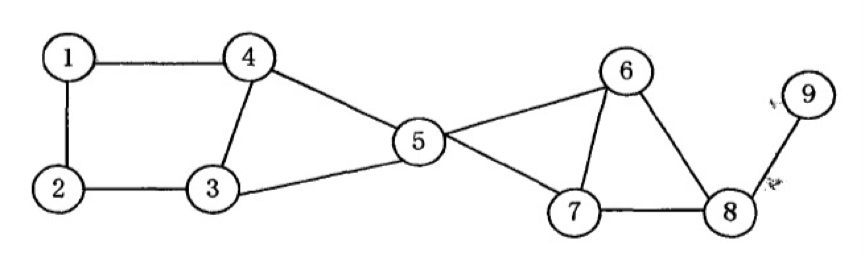
\includegraphics[width=0.75\textwidth]{figures/fig2-2}
  \caption{社交网络中度的幂律分布曲线}\label{fig2-2}
\end{figure}

% \section{社区发现}
\section{社区的定义}

社交网络除了小世界效应和无标度特性这两个典型特征之外,还有一个重要的一个特点就是“社区(Community)”的存在。也有一些学者将之译为“社团”,本文将之称为社区。在直观上,同现实生活中所说的社区一样,社交网络乃至复杂网络中的社区也可以简单地被理解为是一些彼此之间联系紧密的节点的集合,或者说是一些拥有共同或相似属性的个体组成的团体,这些集合或者团体对于分析社交网络有着至关重要的意义。目前在学术界对社区的概念尚且还没有一个完整统一的定义。本文下面从不同的角度给出了三种定义:基于网络拓扑结构的定义、基于节点相似度的定义和重叠社区的定义。

(1)基于网络拓扑结构的社区定义。将社交网络抽象成一个由节点(人或组织)和边(社会关系)组成的网络拓扑结构,那么一个社区就是指由若干个节点组成的具有高内聚特性的子集合。在这个子集合之中的节点彼此之间联系紧密,表现上就是存在着相对比较多的边;而在多个子集合之间,也就是社区之间联系比较稀疏,表现上就是存在着相对较少的边。图\ref{fig:fig2-3}所示即是一个具有社区结构的网络。图中的14个节点组成的网络拓扑图中形成了3个社区结构,为了更直观显示,三个社区的节点分别以黄色、蓝色和绿色三种颜色区分。此种定义对应的社区发现算法即是本文绪论第二小节国内外研究现状中提到的基于链接的社区发现算法。

\begin{figure}
  \centering
  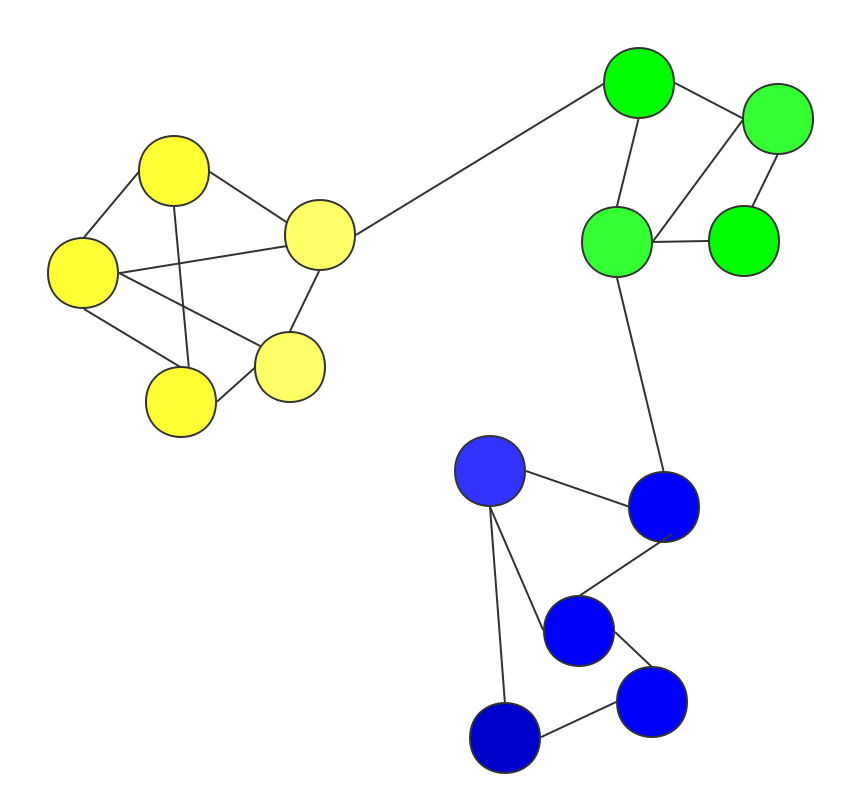
\includegraphics[width=0.75\textwidth]{figures/fig2-3}
  \caption{一个具有社区结构的网络示意图}\label{fig:fig2-3}
\end{figure}

(2)基于节点相似度的社区定义。这里定义的社区依然是由若干节点组成的子集合,但是在表现形式以及定量分析手段上,这与基于网络拓扑结构的定义不同。该定义假定一个社区内部的节点都是相似的,而社区之间的节点的相似度则较低。节点之间的相似度的高低依靠建立节点相似度模型来衡量。这在直观上也不难理解,因为社区本就是代表着社交网络中具有相同或者类似属性的元素的子集。此种定义对应的社区发现算法即是本文绪论第二小节国内外研究现状中提到的基于内容的社区发现算法。

其实在本质上,基于网络拓扑结构的社区定义和基于节点相似度的社区定义是一致的。两者都是将社区定义为网络中所有元素组成的集合的若干子集,在子集之中的元素基于某种因素会彼此连接紧密,而与其他子集内的元素连接稀疏。只不过两者对于元素之间的紧密与稀疏的定量分析手段不同,前者是根据网络的拓扑结构,根据节点之间的边的联系,而后者是根据节点的属性分析节点间相似度。

(3)重叠社区的定义。上文关于社区的定义都忽视了个体可能属于两个或更多社区的可能性。但是,许多真实的社交网络都存在着社区的重叠。例如,一个人可以属于多个社交群体,例如家庭群体和朋友群体。图\ref{fig:fig2-4}所示即是一个具有重叠社区结构的网络。图中的16个节点组成的网络拓扑图中形成了3个社区结构,三个社区的节点分别以黄色、蓝色和绿色三种颜色区分,而这其中有两个黄蓝相间的节点即是同时属于黄色代表的社区和蓝色代表的社区。重叠社区(Overlapping Communities)和普通社区相比,唯一的差别就在于,代表重叠社区的子集之间可以有交集,而代表普通社区的子集之间是没有交集的。而在包含重叠社区的网络中,这些重叠社区间的交集,也就是这些属于多个社区的元素(个体),对社区的演化和社区间的沟通都起到了极其重要的作用,因为它们就是不同社区之间的桥梁和纽带。一般而言,重叠社区结构也可以分为两种。一种是离散型重叠社区,即一个节点要么属于某一个社区,要么不属于这一个社区。另一种是模糊型重叠社区,即每个节点有着对于不同社区的隶属度。关于重叠社区的定义对应的社区发现算法即是本文绪论第二小节国内外研究现状中提到的重叠社区发现算法。

\begin{figure}
  \centering
  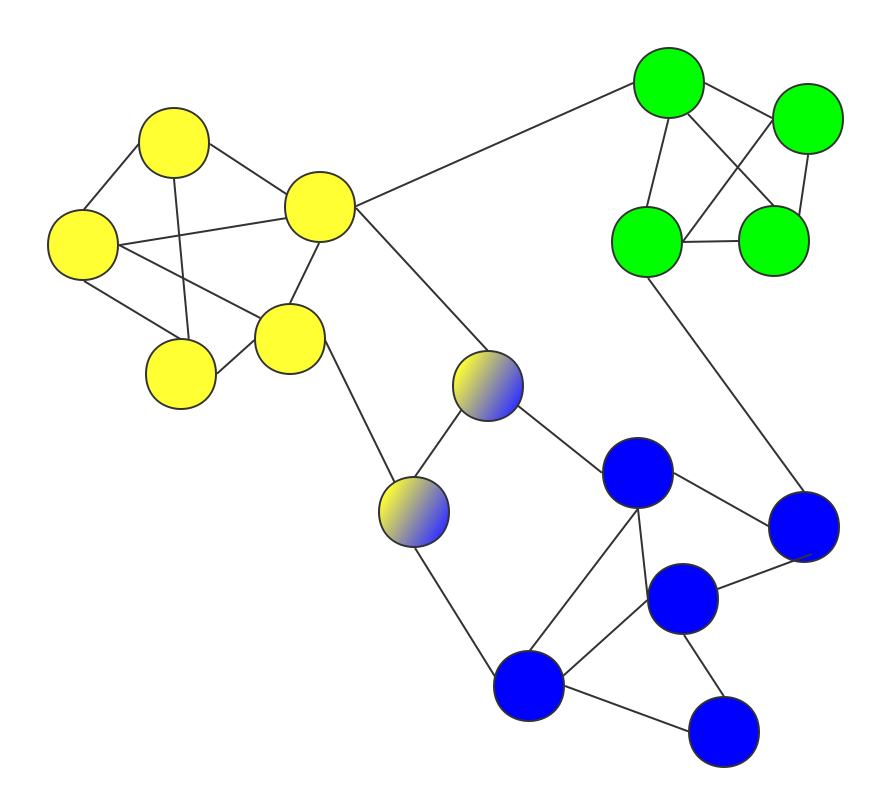
\includegraphics[width=0.75\textwidth]{figures/fig2-4}
  \caption{一个具有重叠社区的网络示意图}\label{fig:fig2-4}
\end{figure}

\section{社区发现}

上一小节已经较为详细的解释了社区的含义。那么给定一个网络图$G=(V,E)$,其中顶点集为$V$,边集为$E$,找出其社区结构的过程就叫做社区发现(Community Detection,也可以译作社区检测)。社区发现是一个复杂而有意义的过程,它对研究社交网络乃至复杂网络的特性具有重要作用。挖掘社交网络中的社区在人物分析、商业个性化推荐和舆情控制等领域有着很关键的作用。
 
在社交网络之中,社区结构是客观存在的,但某个社区内的某个用户只和那些与其有直接边相连的用户产生互动,殊不知在这个社区内,他和那些与其没有直接边相连的用户其实也很“近”,如果要做好友推荐,属于同一社区的用户之间就应该优先进行推荐。此外,“物以类聚,人以群分”,对一个大型网络调用社区发现算法,其实是对其按照某种标准进行了划分,在此基础上可对每个社区做进一步的发掘。而从计算的角度而言,社区划分相当于分解了任务,起到了降低计算复杂度的作用。并且目前的社交软件上用户广泛,不可能将所有用户的信息都存储在同一台服务器之上,这就必须要使用到分布式存储。在分布式存储中,如果不经过分类杂乱无章的进行存储,那么最终将导致巨大的通信开销,而如若先将社交网络进行社区发现,把同一社区内的用户存储在同一服务器内,这就可以省下大笔的通信开销,大大提高社交平台的性能。

近几年,发现及分析社交网络中的社区结构得到了许多学者的关注,同时也出现了很多的社区发现算法,在本文绪论第二小节国内外研究现状中将社区发现算法分为了基于链接的算法、基于内容的算法和融合了链接与内容的算法。在针对社区是否重叠上,还可以将其分为非重叠社区发现和重叠社区发现。对于具体的算法,此处不再赘述。

% \section{本章小结}


% \subsection{社区网络模型描述}

% 网络中社区结构表示的是网络中节点集合的子集。一般情况下,一个复杂的网络可以这样表示:由顶点集 $V$和边集 $E$组成的图$G=(V,E)$。节点个数表示为$n=|V|$,边数表示为$m=|E|$。如果任意两个节点对 $(i, j)$ 与 $(j, i)$表示的是同一条边,该图被称为无向图,否则,该被称为有向图。如果我们给图中的每一条边都设置一个代表关系强弱程度的数值,我们把这种图定义为有权图;否则,该图被称为无权图。显然,我们也可以把无权图看成图中每条边权重值都相同的有权图,比如权值都为1。在无向图中的定义中,节点i的度指的是以i为顶点的边的数目,记为,是所有含有该节点的边的数量的总和。在有向图的定义中,节点的度分为两种类型,入度和出度。以该节点为终点的边的数量为该节点的出入度,以该节点为起点的边的数量为该节点的出度。在无向图中无出入度之分。此外,我们还可以用邻接矩阵或者邻接表来表示网络的真实拓扑结构,邻接矩阵如果是对称矩阵那么表示的是无向图,如果是非对称的矩阵表示就是有向图。

% \section{社区结构评价指标}

% 迄今为止,出现了各种各样的社区发现算法,如何评价不同的的发现算法的好坏是一个非常重要的问题。为此,学者们提出了多种社区结构评价指标用来评价网络社区划分质量,其中比较有代表性的有模块度、NMI等。下面详细介绍这些指标。

% \subsection{模块度}

% 模块度是目前学者们最常用和经典的网络社区结构评价指标,它最初是被Newman等人于2004年提出来的\cite{2002Community}。其通过比较现有网络和基准网络在相同社区划分下的连接密度差来衡量网络社区的优劣,其中基准网络是由原网络具有相同度序列的随机网络。模块度计算方式详见公式\ref{eqn:modular}。

% \begin{equation}
%   \label{eqn:modular}
%   Q=\frac{1}{2m}\sum_{i,j}\left [ A_{ij}-\frac{k_ik_j}{2m} \right ]\delta (c_i, c_j)  
% \end{equation}

% 其中,A 表示网络中的邻接矩阵, m 表示网络中边的总数,$k_i$和$k_j$表示节点 i 和 j 的度数,$c_i$和$c_j$表示节点 i 和 j 所属的社区。如果$i=j,\delta(c_i,c_j)=1$,反之$\delta(c_i,c_j)=0$

% ......

% \subsection{NMI}

% 随着在线社交网络的发展,人们发现在线社交网络的很多数据中存在着暗示各个节点的社区属性信息。例如,在人人网的学校信息便揭示了网络节点中属于同一学校的社区结构,Facebook中的兴趣信息同样表征了具有相同兴趣的虚拟用户群体。这些数据在为社区发现问题提供了丰富的信息的同时,也在一定程度上为虚拟社区结构优劣的评判提供了标准答案。针对这种预先拥有一定虚拟社区结构信息的情况下,Leon Danon等人【34】提出了Normalized Mutual Information(NMI)利用信息化熵来衡量算法划分的社区结构和预先已知的社区结构之间的差异。NMI是基于混合矩阵(Confusion Matrix)N来计算的数字指标。NMI计算方式详见公式\ref{eqn:nmi}。

% \begin{equation}
%   \label{eqn:nmi}
%   NMI=\frac{ -2 \sum_{i,j} N_{ij}  ln{\frac{N_{ij}}{N_iN_j}} } {\sum_{i}N_iln{\frac{N_i}{n}}+\sum_{j}N_jln{\frac{N_j}{n}}}
% \end{equation}

% 使用该数字指标,可以衡量划分出来的社区结构与已知的网络社区结构的差异程度值,该值越大,则表明获得的社区结构划分越好,当该值达到最大化值1时,说明算法发现的社区结构与已知社区结构完全已知,效果最好。

% \begin{figure}
%   \centering
%   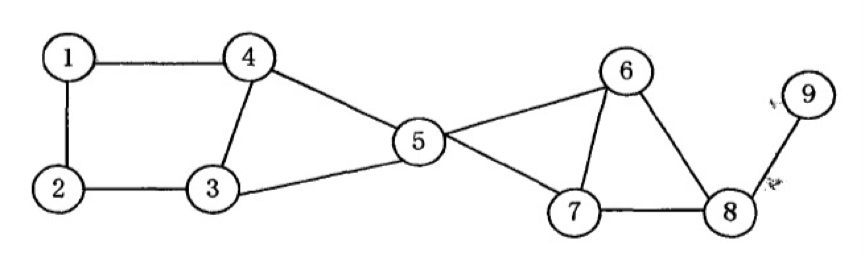
\includegraphics[width=0.75\textwidth]{figures/fig2-2}
%   \caption{网络示例}\label{fig:fig2-2}
% \end{figure}

% 下面以图\ref{fig:fig2-2}为例来说明计算NMI的过程。假设已知的最佳社区结构划分为集合{1,2,3,4}和{5,6,7,8},相应的社区划分向量表示为a = (1,1,1,1,2,3,3,3,3),再假设某算法获得的社区划分结构可以用向量表示为b = (3,3,3,3,2,1,1,1,1)来表示。根据已知的社区划分向量,可以构造混合矩阵\ref{eqn:n}。

% \begin{equation}
%   \label{eqn:n}
%   N=\begin{bmatrix}
%     0 & 0 &4 \\ 
%     0 & 1 & 0\\ 
%     4 & 0 & 0
%     \end{bmatrix}
% \end{equation}

% 根据上式计算可知,该划分的NMI值为1。
